% 原书 p.38–p.42（PDF p.46–p.50）
% >>> p046
\section{矩映射（Moment Map）}

\begin{keytakeaways}
\begin{itemize}
  \item 物理图像：连续对称性的守恒量由矩映射统一给出——$\T^n$ 作用的矩映射即 $n$ 个
        相互对合的守恒量，「角动量」是其最经典的例子。
  \item 数学工具：$\langle\mu(x),v\rangle=H_v(x)$ 的定义（相当于
        $\dd\langle\mu,v\rangle=-\iota_{X_v}\omega$）、极坐标下的标准辛形式、
        Atiyah--Guillemin--Sternberg 凸性定理。
  \item 几何观点：矩映射是作用生成元 $v\mapsto H_v$ 的对偶映射
        $\mathfrak{g}\to C^\infty(M)$ 的对偶；矩像的凸性把辛几何问题化为多面体几何。
  \item 本节结论：$\C^n$ 与 $\CP^2$、$S^2\times S^2$ 上环面作用的矩像分别是
        非负象限与（标准的）单纯形、正方形；由此引出辛环面流形与 Delzant 多面体的
        分类纲领（定义 2.5.2、注 2.5.4）。
\end{itemize}
\end{keytakeaways}

让我们从（角）动量的一般定义出发——简称为\textbf{矩映射}（moment map），作为例 2.4.4
的推广。

\begin{wdefn}{2.5.1}
设 $(M,\omega)$ 是配有 Lie 群 $G$ 的哈密顿群作用的辛流形。该作用的\textbf{矩映射}
是一个映射 $\mu:M\to\mathfrak{g}^*$，它是定义 2.4.2 条件 (i) 中对应关系的对偶，
满足如下条件
\[
  \langle\mu(x),v\rangle=H_v(x)
\]
对任意向量 $v\in\mathfrak{g}$ 与任意点 $x\in M$ 成立。
\end{wdefn}
% [Tutor Note: 这里的 $\langle\cdot,\cdot\rangle:\mathfrak{g}^*\times\mathfrak{g}\to\R$
% 是自然配对。把定义 2.5.1 微分即得等价的无穷小形式
% $\dd\langle\mu,v\rangle=-\iota_{X_v}\omega$——这正是定义 2.4.2 条件 (i) 中对偶的表述；
% 故矩映射的存在性要求每个 $X_v$ 都是哈密顿向量场，而 $\mu$ 的「可积性」要求
% $v\mapsto H_v$ 是 Lie 代数同态（条件 (ii)）。符号约定再次取决于 (2.4)：
% 若把 $\dd H=-\iota_{X_H}\omega$ 换成相反的符号，$\mu$ 也整体变号。]

下面给出几个常见的例子。

% >>> p047
\begin{wexam}{2.5.1}
取 $G=SO(3)$、$(M,\omega)=(T^*\R^3,\omega_{\mathrm{can}})$，其作用如例 2.4.4 所定义。
则其矩映射 $\mu:M\to\mathfrak{so}(3)\,(\cong\R^3)$ 如 (2.26) 那样算得为
$\mu(q,p)=q\times p$。\hfill$//$
\end{wexam}

\begin{wexam}{2.5.2}
考虑 Lie 群 $\T^n$ 作用在 $(\C^n,\omega_{\mathrm{std}})$ 上。标准作用定义为
\begin{equation}
  (t_1,\cdots,t_n)\cdot(z_1,\cdots,z_n)
  =\big(\ee^{\sqrt{-1}t_1}z_1,\cdots,\ee^{\sqrt{-1}t_n}z_n\big),
  \tag{2.27}
\end{equation}
其中 $t_i\in[0,2\pi]$（$1\le i\le n$）。在 $\C^n$ 上计算矩映射 $\mu$ 的最佳途径是
用极坐标下的 $\omega_{\mathrm{std}}$，即
\begin{equation}
  \omega_{\mathrm{std}}=\sum_{i=1}^nr_i\,\dd r_i\wedge\dd\theta_i,
  \tag{2.28}
\end{equation}
其中 $r_i>0$、$\theta_i\in[0,2\pi]$（$1\le i\le n$）。对
$v=(1,0,\cdots,0)\in\R^n\,(=\mathfrak{g})$，有 $\exp(tv)=(t,0,\cdots,0)$，于是在任意点
$(r_1,\theta_1,\cdots,r_n,\theta_n)$ 处有
\begin{align*}
  \left.\frac{\dd}{\dd t}\exp(tv)(r_1,\theta_1,\cdots,r_n,\theta_n)\right|_{t=0}
  &=\left.\frac{\dd}{\dd t}(r_1,\theta_1+t,\cdots,r_n,\theta_n)\right|_{t=0}\\
  &=(0,1,0,\cdots,0)=X_v(r_1,\theta_1,\cdots,r_n,\theta_n).
\end{align*}
由定义 2.4.2，可知 $H_v(r_1,\theta_1,\cdots,r_n,\theta_n)=\dfrac12r_1^2$。因此该
$\T^n$-作用的矩映射为
\begin{equation}
  \mu(z_1,\cdots,z_n)
  =\Big(\frac12|z_1|^2,\cdots,\frac12|z_n|^2\Big)\in\R^n_{\ge0},
  \tag{2.29}
\end{equation}
它满足
$\langle\mu(z_1,\cdots,z_n),v\rangle=H_v(r_1,\theta_1,\cdots,r_n,\theta_n)$。\hfill$//$
\end{wexam}
% [Tutor Note: (2.28) 中 $\omega_{\mathrm{std}}=\sum r_i\,\dd r_i\wedge\dd\theta_i$ 与
% 直角坐标下的 $\sum\dd x_i\wedge\dd y_i$ 一致（$x=r\cos\theta,\ y=r\sin\theta$ 时
% $\dd x\wedge\dd y=r\,\dd r\wedge\dd\theta$）。注意原书把这一坐标下的动量记为
% $(0,1,0,\cdots,0)$，即 $\partial_{\theta_1}$；由 $\iota_{\partial_\theta}(r\,\dd r\wedge
% \dd\theta)=-r\,\dd r$ 得 $H_v=\frac12r_1^2$，与 $-\iota_{X_v}\omega=\dd H_v$ 相符。
% 另注：原文 (2.29) 末句多了一个右括号，属排版笔误。]

\begin{wrem}{2.5.1}
定义 2.5.1 中的哈密顿函数 $H_v$ 一般而言并不唯一，两个这样的哈密顿函数相差一个常数。
于是所得的矩映射 $\mu$ 将是 (2.29) 在 $\R^n$ 中的一个平移。
\end{wrem}

\begin{wexam}{2.5.3}
考虑 $\T^2$ 在 $(\CP^2,\omega_{\mathrm{FS}})$ 上的作用，定义为
\[
  (t_1,t_2)\cdot[z_0,z_1,z_2]
  =\big[z_0,\ee^{\sqrt{-1}t_1}z_1,\ee^{\sqrt{-1}t_2}z_2\big],
\]
其中 $(t_1,t_2)\in S^1\times S^1=\T^2$，$[z_0,z_1,z_2]\in\CP^2$。与上面的例 2.5.2
类似，其矩映射计算如下
\begin{equation}
  \mu([z_0,z_1,z_2])
  =\frac12\left(
    \frac{|z_1|^2}{\sum_{i=0}^2|z_i|^2},
    \frac{|z_2|^2}{\sum_{i=0}^2|z_i|^2}
  \right).
  \tag{2.30}
\end{equation}
与 (2.29)（其中 $\mu$ 的像是整个 $\R^n_{\ge0}$）不同，(2.30) 中 $\mu$ 的像是一个
有界区域（这是除以 $\sum_{i=0}^2|z_i|^2$ 所致）。
% >>> p048
画出 (2.30) 中矩映射 $\mu$ 的像的一个办法，是从上述作用的不动点出发。共有三个不动点：
$[1,0,0]$、$[0,1,0]$ 与 $[0,0,1]$。于是得到下图，即图 2.4，其中阴影区域是 $\mu$ 的像。
注意 $\mu$ 的这个像是标准的二维单纯形，特别地它是凸的，且其顶点恰好是群作用的不动点。
\hfill$//$
\end{wexam}

\begin{figure}[htbp]
  \centering
  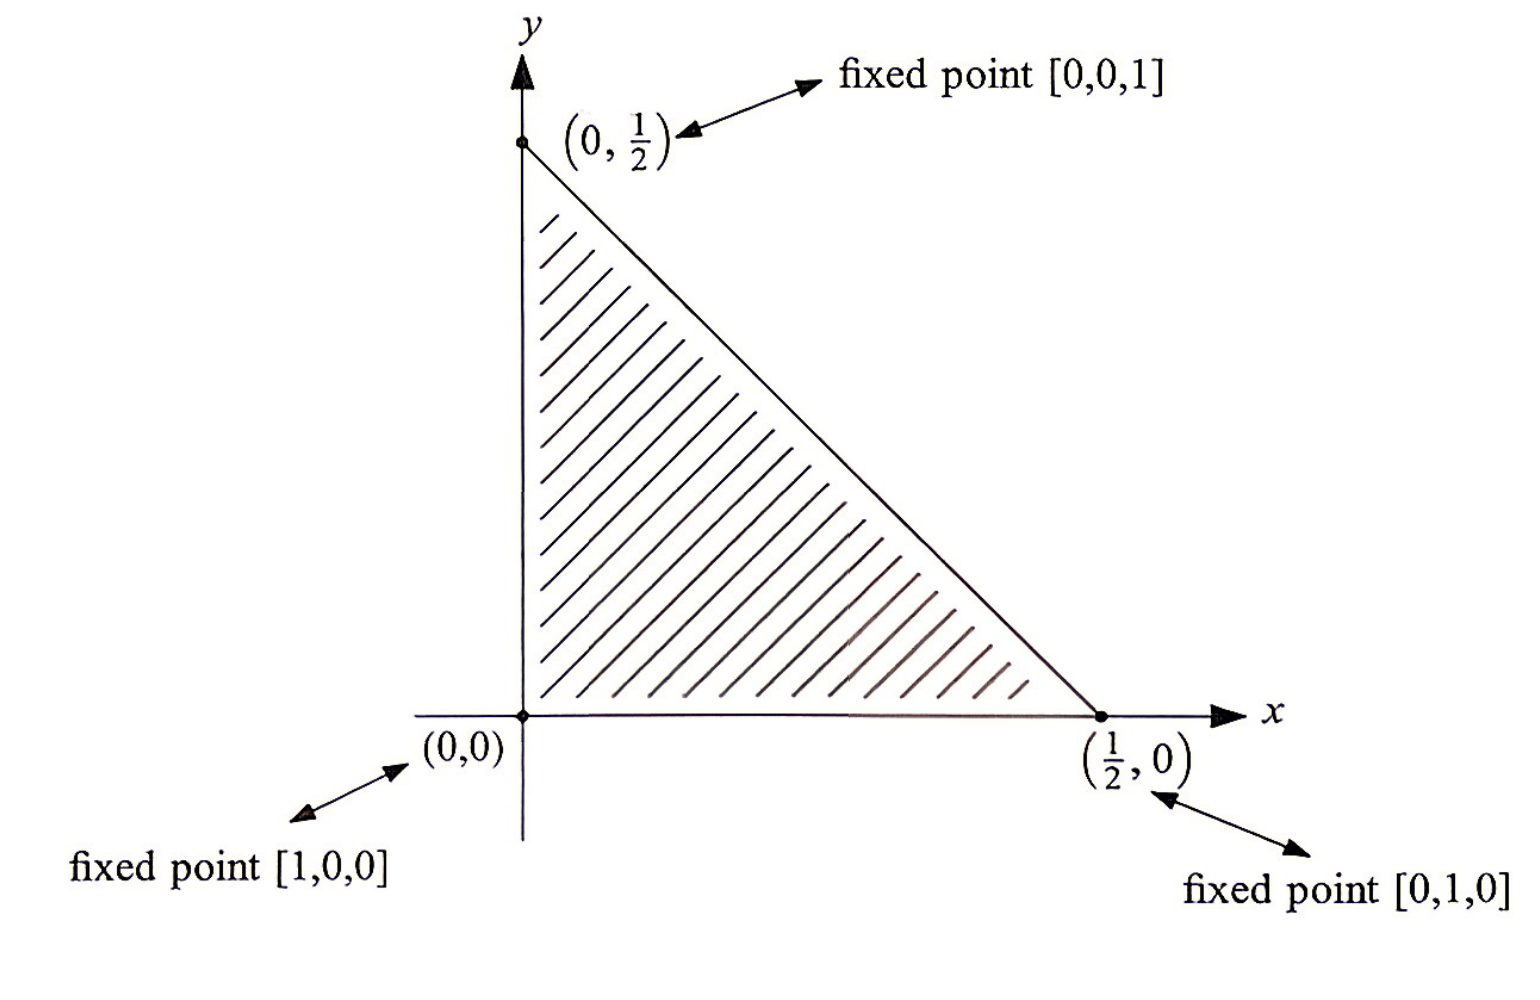
\includegraphics[width=0.62\linewidth]{figures/fig_p048_1.png}
  \caption*{图 2.4\quad 群作用 $\T^2\curvearrowright(\CP^2,\omega_{\mathrm{FS}})$ 的
  矩映射之像（原书 p.40, Figure 2.4；PDF p.48）}
\end{figure}

\begin{wrem}{2.5.2}
例 2.5.3 中 $\T^2$ 在 $\CP^2$ 上的作用也是有效的。我们来核对 $[1,1,1]$ 处的稳定
化子。若 $(t_1,t_2)\cdot[1,1,1]=[1,\ee^{\sqrt{-1}t_1},\ee^{\sqrt{-1}t_2}]=[1,1,1]$，
则 $t_1=t_2=0$，即 $\T^2$ 中的单位元。
\end{wrem}

\begin{wexam}{2.5.4}
考虑 $\T^2$ 在 $(S^2\times S^2,\omega_{\mathrm{prod}})$ 上的作用，定义为
\[
  (t_1,t_2)\cdot\big([z_0,z_1],[w_0,w_1]\big)
  =\Big(\big[z_0,\ee^{\sqrt{-1}t_1}z_1\big],\big[w_0,\ee^{\sqrt{-1}t_2}w_1\big]\Big).
\]
则矩映射计算为
\[
  \mu\big([z_0,z_1],[w_0,w_1]\big)
  =\frac12\left(
    \frac{|z_1|^2}{|z_0|^2+|z_1|^2},
    \frac{|w_1|^2}{|w_0|^2+|w_1|^2}
  \right).
\]
与例 2.5.3 类似，若考虑此作用的不动点——共有四个，即 $([0,1],[0,1])$、
$([0,1],[1,0])$、$([1,0],[0,1])$ 与 $([1,0],[1,0])$——则 $\mu$ 在 $\R^2_{\ge0}$ 中的
像由图 2.5 给出。
% >>> p049
再次注意，这个像是凸的，且其顶点恰为该作用的不动点。\hfill$//$
\end{wexam}

\begin{figure}[htbp]
  \centering
  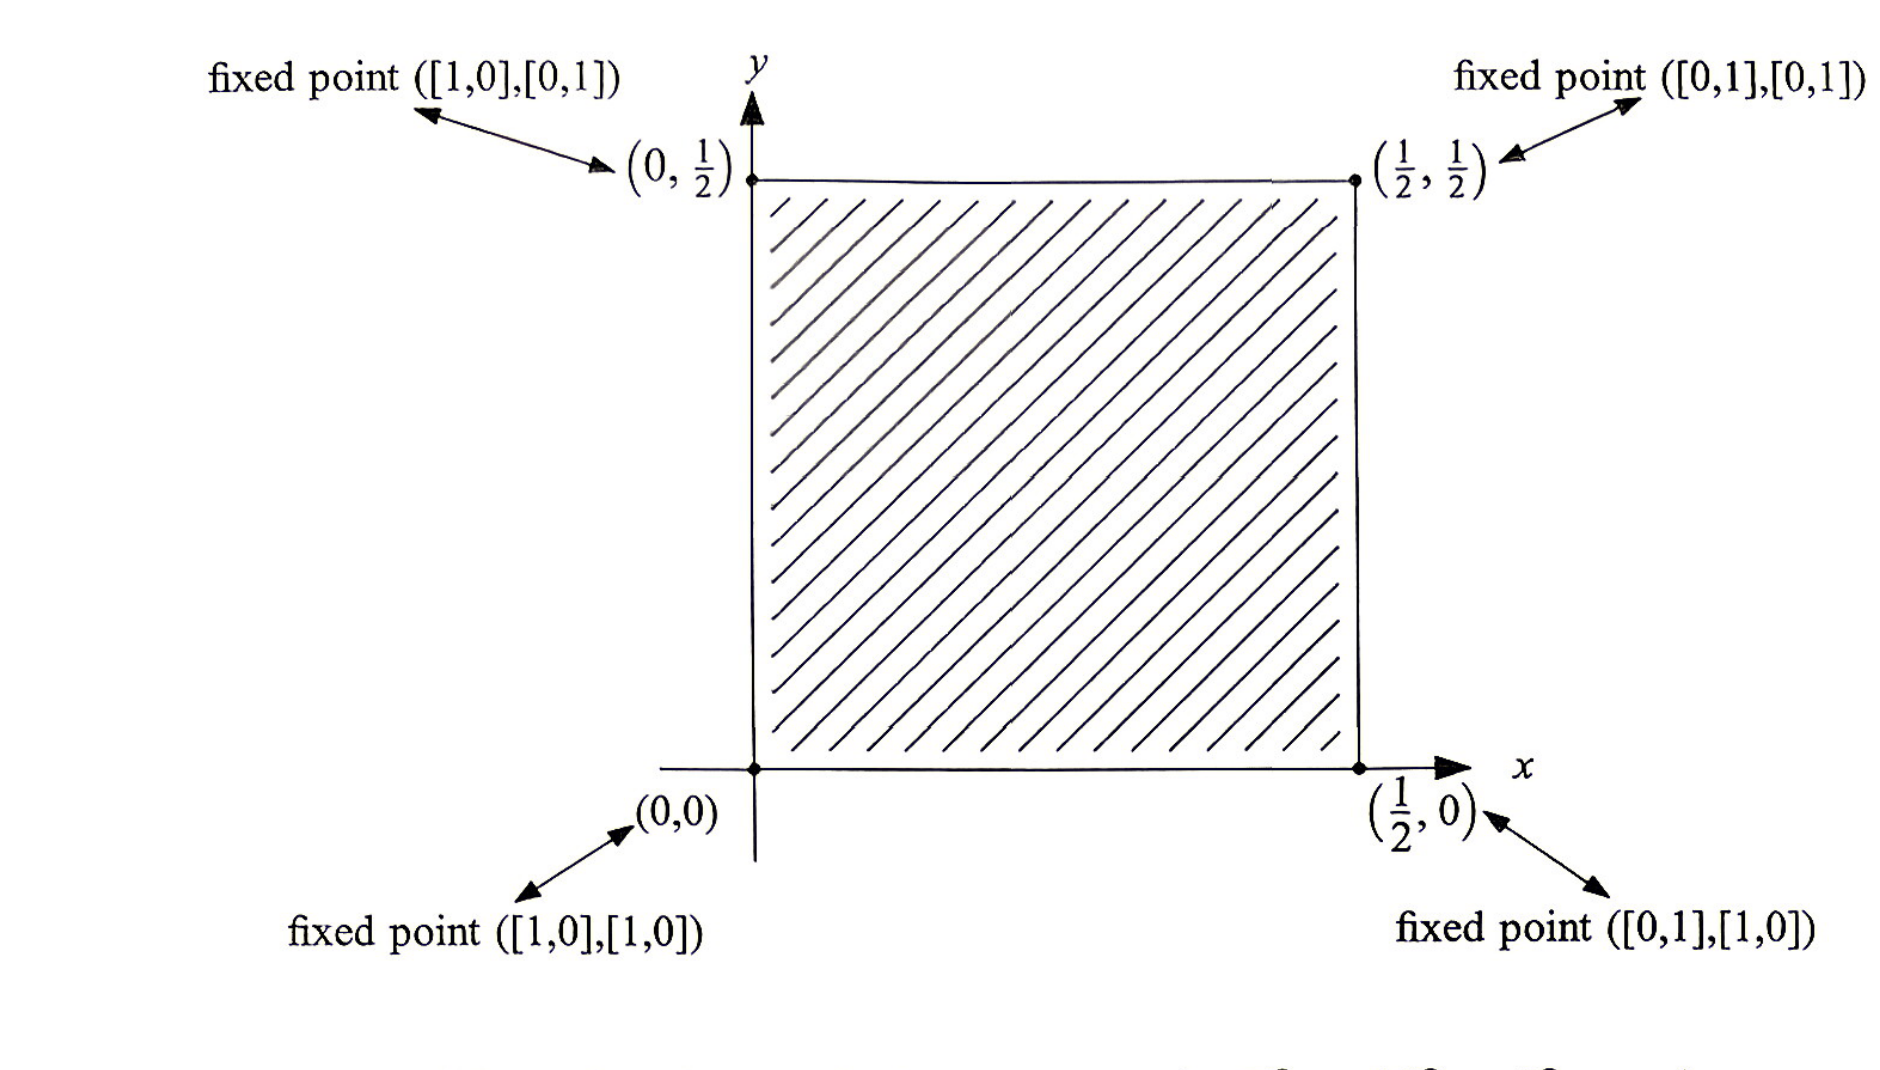
\includegraphics[width=0.66\linewidth]{figures/fig_p049_1.png}
  \caption*{图 2.5\quad 群作用 $\T^2\curvearrowright(S^2\times S^2,
  \omega_{\mathrm{prod}})$ 的矩映射之像（原书 p.41, Figure 2.5；PDF p.49）}
\end{figure}

例 2.5.3 与例 2.5.4 中矩映射之像所共有的性质，事实上可由如下结果确认。

\begin{wthm}{2.5.1}
（Atiyah--Guillemin--Sternberg [18,103]）设 $(M,\omega)$ 是配有哈密顿 $\T^n$-作用的
闭辛流形。则关于矩映射与矩像的性质，如下结论成立。
\begin{enumerate}[label=(\roman*)]
  \item 该作用下的不动点集是有限个两两不交的连通子流形之并
        $\bigsqcup_iQ_i$，且 $\omega|_{Q_i}\equiv0$。
  \item 将 $\mu$ 限制到每个 $Q_i$ 上，记 $\mu|_{Q_i}=\lambda_i\in\R^n$。换言之，
        $\mu|_{Q_i}$ 是常值函数。
  \item $\mu$ 在 $\R^n$ 中的像记作 $\operatorname{im}(\mu)$，它是凸多胞形。更确切地说，
        \[
          \operatorname{im}(\mu)
          =\Big\{\sum_ix_i\lambda_i\ \Big|\ \sum_ix_i=1,\ x_i\ge0\Big\},
        \]
        即向量 $\lambda_i$ 的凸包，其中 $\lambda_i$ 来自上面 (ii)。
\end{enumerate}
\end{wthm}
% [Tutor Note: 原文疑误——(i) 中「a finite union of pairwise disjoint connected of
% submanifolds」多出一个 of，应为「connected submanifolds」；(iii) 中的
% $\operatorname{im}(u)$ 应为 $\operatorname{im}(\mu)$。译文照原文语义处理，详见
% review_ch02.md。另注：本定理要求 $M$ 闭（紧且无边界）且作用为哈密顿的；
% 不动点分支 $Q_i$ 是迷向子流形（$\omega|_{Q_i}\equiv0$），其维数不超过 $\dim M/2$，
% 这正是下段所说「当 $n<\frac12\dim M$ 时会出现高维 $Q_i$」的来源。]

在上面的例子中，我们总有 $Q_i$ 为点（从而定理 2.5.1 的结论 (ii) 平凡地成立）。若
$n=\dim\T^n<\dfrac12\dim M$，则可能出现更高维的子流形 $Q_i$（参见 [49] 中的例 4.17）。

\begin{wrem}{2.5.3}
上述定理\emph{不}要求 $\T^n$-作用是有效的。
\end{wrem}

\begin{wexer}{2.5.1}
（例 4.15 (4)$^{[49]}$）考虑如下辛流形
\[
  M=\big\{([a,b],[x,y,z])\in\CP^1\times\CP^2\mid ay=bx\big\},
\]
配有乘积辛结构 $\omega_{\mathrm{prod}}$，并由下式定义 $\T^2$ 在
$(M,\omega_{\mathrm{prod}}|_M)$ 上的作用：
\[
  (t_1,t_2)\cdot\big([a,b],[x,y,z]\big)
  =\Big(\big[\ee^{\sqrt{-1}t_1}a,b\big],
  \big[\ee^{\sqrt{-1}t_1}x,y,\ee^{\sqrt{-1}t_2}z\big]\Big).
\]
% >>> p050
计算矩映射 $\mu$，并求出此作用的不动点。
\end{wexer}

至此，我们主要关注的是 $\T^n$ 在 $(M,\omega)$ 上的作用。由这一研究自然产生了一个新的
定义，它在辛几何领域已被广泛使用。

\begin{wdefn}{2.5.2}
\textbf{辛环面流形}（symplectic toric manifold）是指配有有效哈密顿环面作用 $\T^n$ 的
辛流形 $(M^{2n},\omega)$。
\end{wdefn}

\begin{wrem}{2.5.4}
定义 2.5.2 的关键在于维数关系：$\dim\T^n=\dfrac12\dim M^{2n}$。回顾例 2.4.3 的第二
部分，若 $(M,\omega)$ 容许 $\T^n$ 的有效哈密顿环面作用，则 $\dim M\ge2n$。因此，辛环面
流形被定义为这一最小维数的情形。
\end{wrem}
% [Tutor Note: 「辛环面流形」与代数几何中的（经典）环面簇（toric variety）是不同范畴的
% 对象：前者是辛流形加 $\T^n$-作用，后者是复代数簇加 $(\C^*)^n$-作用；Delzant 的定理通过
% 矩多面体把二者联系起来。术语依据：toric 在辛几何文献中通行译作「环面的」，
% moment polytope 译「矩多面体」。]

关于辛环面流形的一个漂亮结论是：它们可以由其矩像（称为 \textbf{Delzant 多面体}）
分类。特别地，若两个辛环面流形在其矩映射下有相同的像，则它们之间存在 $\T^n$-等变的
辛同胚。更多细节见 [40] 第 I 章以及 T. Delzant 的原始论文 [64]；在那里还可了解辛环面
流形与代数几何中（经典）环面簇之间的关系。
